\documentclass[12pt,a4paper]{article}
\usepackage[utf8]{inputenc}
\usepackage[T1]{fontenc}
\usepackage{geometry}
\usepackage{amsmath}
\usepackage{amsfonts}
\usepackage{subcaption}
\usepackage[labelfont=bf]{caption}
\usepackage{amssymb}
\usepackage{graphicx}
\usepackage{float}
\usepackage{cite}
\usepackage{url}
\usepackage{hyperref}
\usepackage{subfigure}
\usepackage{booktabs}
\usepackage{multirow}
\usepackage{algorithm}
\usepackage{algorithmic}
\usepackage{listings}
\usepackage{xcolor}

\geometry{margin=1in}

\title{Uso di tecniche di LLM per analizzare traiettorie turistiche e per suggerire la prossima attrazione turistica da visitare}

\author{
Simone Mattioli\\
Department of Computer Science\\
University of Verona\\
}
\date{\today}

\begin{document}

\maketitle

\begin{abstract}
This paper presents a comprehensive study on leveraging Large Language Models (LLMs) for predicting human mobility patterns in urban tourism contexts. We introduce LLM-Mob, a novel framework that utilizes the natural language understanding capabilities of modern LLMs to predict tourists' next Points of Interest (POI) based on their historical visiting patterns. Our approach is evaluated on the VeronaCard dataset, which contains real-world tourism data from Verona, Italy, spanning multiple years. We investigate the impact of different contextual information types on prediction accuracy, including basic POI names, geographical coordinates, and temporal features. The framework demonstrates the potential of LLMs to understand complex spatial-temporal patterns in human mobility without requiring extensive feature engineering or domain-specific architectures. Our implementation replaces traditional OpenAI GPT models with open-source Llama 3.1, making the approach more accessible and cost-effective for research purposes.
\end{abstract}

\section{Introduction}

Human mobility prediction has emerged as a crucial research area with applications spanning urban planning, transportation systems, recommendation systems, and public health. Traditional approaches to mobility prediction have relied heavily on statistical models, machine learning algorithms, and deep learning architectures specifically designed for sequential data. However, recent advances in Large Language Models (LLMs) have opened new avenues for understanding and predicting human behavior patterns through natural language processing capabilities.

The fundamental challenge in human mobility prediction lies in capturing the complex interplay between spatial, temporal, and behavioral factors that influence individual movement decisions. Traditional machine learning approaches often require extensive feature engineering and domain-specific knowledge to encode these relationships effectively. In contrast, LLMs possess inherent capabilities for understanding contextual relationships and patterns, which can be leveraged to predict mobility patterns through carefully designed prompts and contextual information.

This paper introduces LLM-Mob, a framework that harnesses the power of Large Language Models for human mobility prediction in tourism contexts. Our approach differs from conventional methods by treating mobility prediction as a natural language understanding task, where historical visiting patterns, geographical information, and temporal context are encoded as textual prompts for LLM inference.

The primary contributions of this work include:

\begin{itemize}
\item A novel framework for human mobility prediction using Large Language Models that requires minimal feature engineering
\item Comprehensive evaluation of different contextual information types on prediction accuracy
\item Implementation using open-source Llama 3.1 models, eliminating dependencies on proprietary APIs
\item Extensive experiments on real-world tourism data from the VeronaCard dataset
\item Analysis of the impact of geographical proximity and temporal patterns on mobility prediction performance
\end{itemize}

\section{Related Work}

Human mobility prediction has been extensively studied across multiple disciplines, with approaches ranging from statistical models to deep learning architectures. Early works focused on Markov-based models that captured transition probabilities between locations based on historical patterns. More recent approaches have leveraged recurrent neural networks (RNNs), Long Short-Term Memory (LSTM) networks, and attention mechanisms to model sequential dependencies in mobility data.

Graph-based approaches have gained prominence due to their ability to capture spatial relationships between locations. These methods typically represent locations as nodes in a graph, with edges encoding spatial proximity or transition probabilities. However, such approaches often require extensive preprocessing and domain-specific feature engineering to achieve satisfactory performance.

The emergence of Large Language Models has introduced new possibilities for mobility prediction. Recent works have explored the use of LLMs for various spatial-temporal tasks, demonstrating their ability to understand geographical relationships and temporal patterns through natural language descriptions. Our work builds upon these foundations by specifically focusing on tourism mobility prediction and investigating the impact of different contextual information types.

\section{Methodology}

\subsection{Problem Formulation}

We formulate the human mobility prediction problem as follows: Given a tourist's historical sequence of visited POIs $S = \{p_1, p_2, ..., p_n\}$ ordered by visit time, we aim to predict the next POI $p_{n+1}$ that the tourist is likely to visit. Each POI $p_i$ is characterized by its name, geographical coordinates (latitude and longitude), and temporal information (visit timestamp).

The prediction task is approached as a natural language generation problem, where the LLM is provided with contextual information about the tourist's behavior and asked to generate the most likely next destinations.

\subsection{Dataset Description}

Our experiments are conducted on the VeronaCard dataset, which contains real-world tourism data from Verona, Italy.\\ The dataset encompasses visitor logs from 2014 to 2023, capturing tourist interactions with various cultural and historical sites throughout the city. The dataset includes:

\begin{itemize}
\item Tourist card usage logs with timestamps and POI identifiers
\item A comprehensive catalog of Points of Interest with geographical coordinates ( In Verona )
\end{itemize}

The POI catalog includes major tourist attractions such as Arena di Verona, Casa di Giulietta and Castelvecchio Museum, among others. Each POI is associated with precise geographical coordinates, enabling spatial analysis of tourist movement patterns.

\subsection{Data Preprocessing and Clustering}

Our preprocessing pipeline consists of several stages designed to clean and structure the raw mobility data:

\subsubsection{Data Cleaning and Filtering}
Raw visitor logs are processed to extract relevant information including visit timestamps, POI names, and tourist card identifiers. We filter out incomplete records and focus on tourists with multiple POI visits to ensure meaningful sequence analysis.

\subsubsection{User Clustering}
To capture behavioral patterns among tourists, we employ K-means clustering on user-POI interaction matrices. The clustering process involves:

\begin{enumerate}
\item Construction of a user-POI matrix where each row represents a tourist and each column represents a POI
\item Standardization of the matrix using StandardScaler to ensure equal weighting of features
\item Application of K-means clustering with $k=7$ clusters to group tourists with similar visiting patterns
\end{enumerate}

This clustering approach enables the identification of distinct tourist profiles, such as culture-focused visitors, history enthusiasts, or casual tourists, which can inform the prediction process.

\section{Prompting Strategies and Experimental Results}

The efficacy of Large Language Models (LLMs) in next-POI prediction is fundamentally dependent on the design of context-aware prompting strategies that effectively encode spatio-temporal mobility patterns. Our experimental framework systematically evaluates three distinct prompting paradigms, each progressively incorporating additional contextual dimensions to assess their impact on recommendation accuracy.

\subsection{Prompting Strategy Taxonomy}

We define three hierarchical prompting strategies, each building upon the previous one to evaluate the incremental contribution of different contextual features:

\begin{enumerate}

\item \textbf{Baseline Strategy (POI Name Only):} The foundational approach provides the model with a chronologically ordered sequence of previously visited POIs represented solely by their canonical names. This strategy serves as our baseline, focusing purely on sequential patterns without any additional contextual information.

\begin{figure}[H]
\centering
\textbf{Confusion Matrix - Baseline Strategy}\par
\vspace{0.5em}
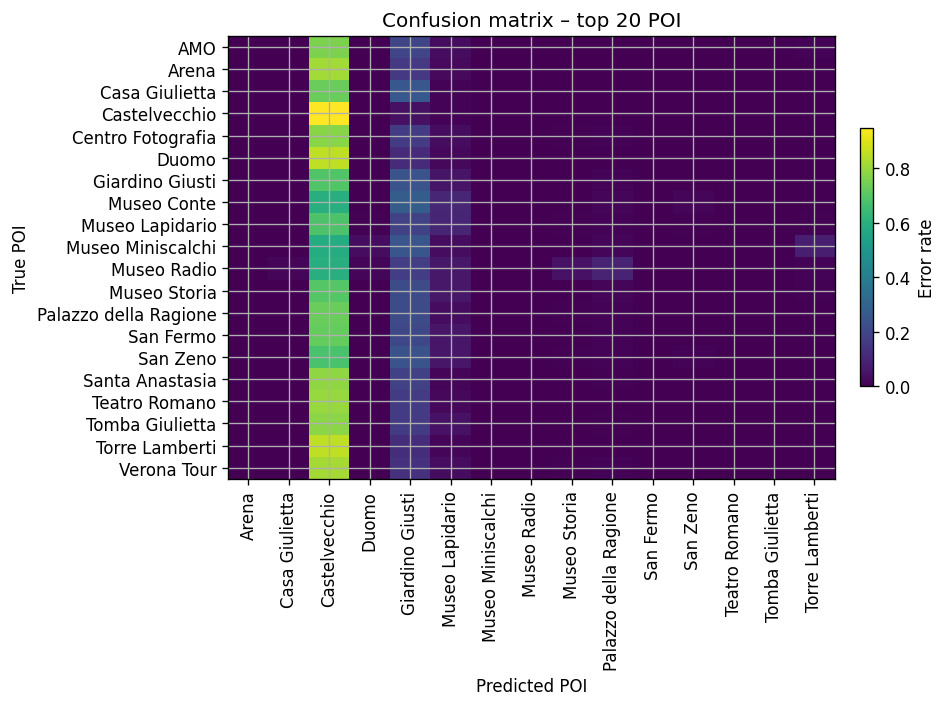
\includegraphics[width=0.8\textwidth]{../img/no_SPACE-GEO_n-1_come_current_POI/confusion_matrix.png}
\caption{The confusion matrix illustrates the misclassification rates between the top 20 most visited POIs in Verona under the baseline strategy. Brighter colors indicate higher confusion. Notably, Castelvecchio is frequently mispredicted as the next POI, reflecting strong sequential bias or user preference patterns.
}
\label{fig:baseline_confusion}
\end{figure}

\begin{figure}[H]
\centering
\textbf{MRR Distribution - Baseline Strategy}\par
\vspace{0.5em}
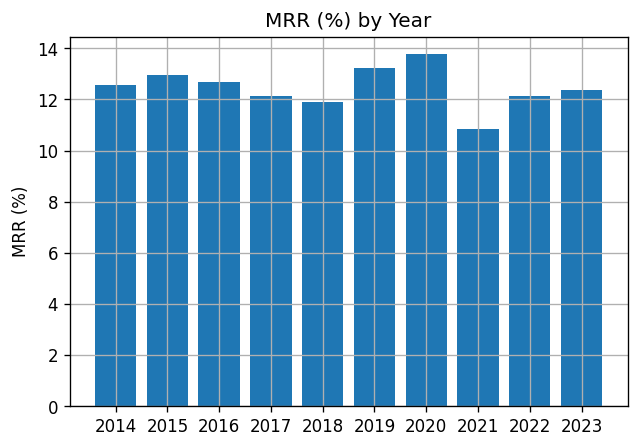
\includegraphics[width=0.8\textwidth]{../img/no_SPACE-GEO_n-1_come_current_POI/mrr_distribution.png}
\caption{The chart shows the Mean Reciprocal Rank (MRR) performance per year showing how well the model ranks the correct POI.. The values fluctuate between 11\% and 14\%, with a noticeable peak in 2020 and a dip in 2021—likely reflecting pandemic-related disruptions in tourist behavior. The trend suggests a generally stable predictive performance over time, with modest variance.
}
\label{fig:baseline_mrr}
\end{figure}

\begin{figure}[H]
\centering
\textbf{Top-1 Accuracy - Baseline Strategy}\par
\vspace{0.5em}
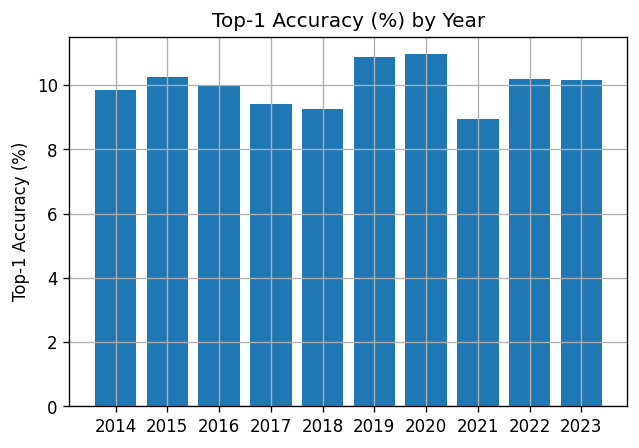
\includegraphics[width=0.8\textwidth]{../img/no_SPACE-GEO_n-1_come_current_POI/top1_accuracy.png}
\caption{Top-1 accuracy score indicating the proportion of times the correct POI was the top prediction.\\ The values hover between 9\% and 11\%, with the highest accuracy observed in 2019/2020 and a significant drop in 2021, likely due to atypical tourist patterns during the COVID-19 pandemic.\\ The performance trend indicates a consistent but modest ability of the model to identify the correct POI as the top prediction.
}
\label{fig:baseline_top1}
\end{figure}

\begin{figure}[H]
\centering
\textbf{Top-5 Hit Rate - Baseline Strategy}\par
\vspace{0.5em}
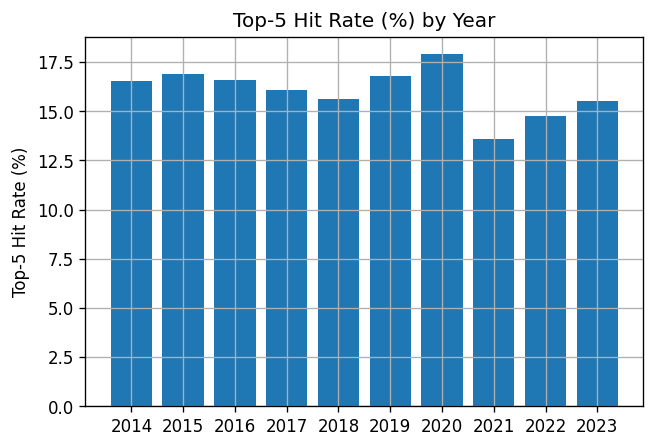
\includegraphics[width=0.8\textwidth]{../img/no_SPACE-GEO_n-1_come_current_POI/top5_hit_rate.png}
\caption{Percentage of predictions where the correct POI appears among the top 5 suggested POIs. ( NO order considered in the top 5)}
\label{fig:baseline_top5}
\end{figure}

\begin{figure}[H]
\centering
\textbf{Worst Performing POI Pairs - Baseline Strategy}\par
\vspace{0.5em}
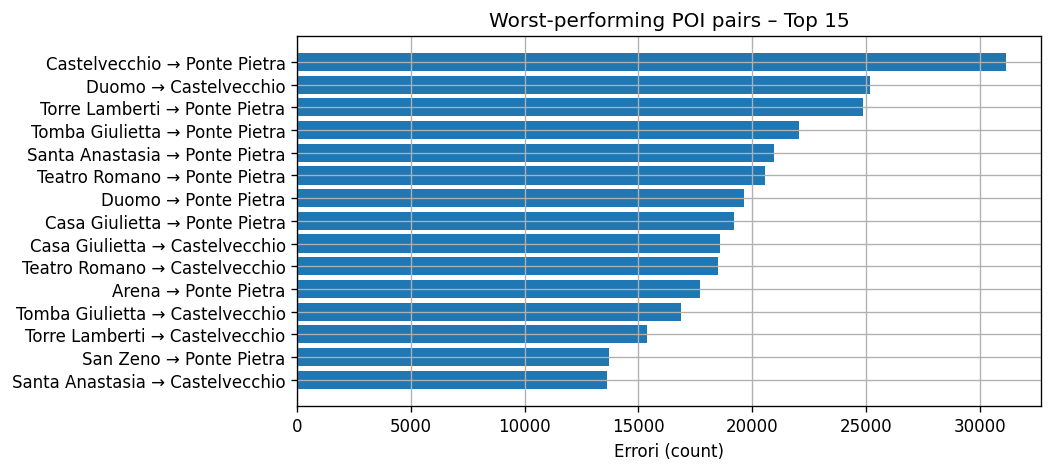
\includegraphics[width=0.8\textwidth]{../img/no_SPACE-GEO_n-1_come_current_POI/worst_performing_pairs.png}
\caption{Pairs of POIs that are most commonly mispredicted, providing insight into frequent confusion cases.}
\label{fig:baseline_worst_pairs}
\end{figure}

\item \textbf{Geospatial-Enhanced Strategy (Name + Geolocation):} This strategy enriches each POI with precise geographic coordinates, allowing the model to leverage spatial patterns.

\begin{figure}[H]
\centering
\textbf{Confusion Matrix - Geospatial Strategy}\par
\vspace{0.5em}
\includegraphics[width=0.8\textwidth]{../img/}
\caption{Confusion matrix showing prediction performance when spatial coordinates are included.}
\label{fig:geospatial_confusion}
\end{figure}

\begin{figure}[H]
\centering
\textbf{MRR Distribution - Geospatial Strategy}\par
\vspace{0.5em}
\includegraphics[width=0.8\textwidth]{../img/your_image_2.png}
\caption{Distribution of MRR scores when geolocation is integrated into the input.}
\label{fig:geospatial_mrr}
\end{figure}

\begin{figure}[H]
\centering
\textbf{Top-1 Accuracy - Geospatial Strategy}\par
\vspace{0.5em}
\includegraphics[width=0.8\textwidth]{../img/your_image_3.png}
\caption{Accuracy of top-ranked predictions under the geospatial-enhanced strategy.}
\label{fig:geospatial_top1}
\end{figure}

\begin{figure}[H]
\centering
\textbf{Top-5 Hit Rate - Geospatial Strategy}\par
\vspace{0.5em}
\includegraphics[width=0.8\textwidth]{../img/your_image_4.png}
\caption{Hit rate for top-5 POIs when spatial data is considered.}
\label{fig:geospatial_top5}
\end{figure}

\begin{figure}[H]
\centering
\textbf{Worst Performing POI Pairs - Geospatial Strategy}\par
\vspace{0.5em}
\includegraphics[width=0.8\textwidth]{../img/your_image_5.png}
\caption{Most error-prone POI transitions despite spatial awareness.}
\label{fig:geospatial_worst_pairs}
\end{figure}

\item \textbf{Comprehensive Context Strategy (Name + Geolocation + Temporal Context):} This approach includes spatial and temporal features, offering the model full spatio-temporal information.

\begin{figure}[H]
\centering
\textbf{Confusion Matrix - Comprehensive Strategy}\par
\vspace{0.5em}
\includegraphics[width=0.8\textwidth]{../img/your_image_6.png}
\caption{Confusion matrix using both spatial and temporal information for POI prediction.}
\label{fig:comprehensive_confusion}
\end{figure}

\begin{figure}[H]
\centering
\textbf{MRR Distribution - Comprehensive Strategy}\par
\vspace{0.5em}
\includegraphics[width=0.8\textwidth]{../img/your_image_7.png}
\caption{MRR distribution reflecting model ranking effectiveness under full context.}
\label{fig:comprehensive_mrr}
\end{figure}

\begin{figure}[H]
\centering
\textbf{Top-1 Accuracy - Comprehensive Strategy}\par
\vspace{0.5em}
\includegraphics[width=0.8\textwidth]{../img/your_image_8.png}
\caption{Top-1 accuracy of the model using complete spatio-temporal context.}
\label{fig:comprehensive_top1}
\end{figure}

\begin{figure}[H]
\centering
\textbf{Top-5 Hit Rate - Comprehensive Strategy}\par
\vspace{0.5em}
\includegraphics[width=0.8\textwidth]{../img/your_image_9.png}
\caption{Hit rate within top-5 predictions using the full contextual strategy.}
\label{fig:comprehensive_top5}
\end{figure}

\begin{figure}[H]
\centering
\textbf{Worst Performing POI Pairs - Comprehensive Strategy}\par
\vspace{0.5em}
\includegraphics[width=0.8\textwidth]{../img/your_image_10.png}
\caption{Difficult POI pairs under the most advanced strategy, despite temporal and spatial modeling.}
\label{fig:comprehensive_worst_pairs}
\end{figure}

\end{enumerate}


\subsection{Experimental Protocol}

Our evaluation employs a systematic approach utilizing the VeronaCard dataset, which provides comprehensive tourist mobility traces across multiple years (2014-2020). The experimental protocol incorporates the following key components:

\begin{itemize}
\item \textbf{Clustering-based User Segmentation:} Tourist behaviors are segmented using K-means clustering (k=7) applied to user-POI interaction matrices, enabling cluster-specific prompting strategies.
\item \textbf{Anchor-based Sequence Construction:} We implement a configurable anchor selection mechanism (\texttt{DEFAULT\_ANCHOR\_RULE = "penultimate"}) to determine the reference point for next-POI prediction within user trajectories.
\item \textbf{Distance-aware POI Ranking:} Geospatial prompts incorporate Haversine distance calculations to rank available POIs by proximity to the current location, reflecting realistic mobility constraints.
\end{itemize}

The prompting mechanism dynamically generates context-aware queries following this template structure:

\begin{lstlisting}[language=text, caption=Comprehensive Context Prompt Template]
Sei un assistente turistico esperto di Verona con conoscenza 
dettagliata della geografia della città.

<cluster_id>: {cluster_id}
<history>: {history}
<current_poi>: {current_poi}

<pois_disponibili_con_distanze>:
{pois_with_distance_text}

Obiettivo: suggerisci i {top_k} POI più probabili che 
l'utente visiterà dopo, considerando:
- La distanza dal POI attuale
- La logica dei percorsi turistici a Verona
- I pattern tipici di movimento in base al cluster {cluster_id}
\end{lstlisting}

\subsection{Evaluation Metrics}

We employ a comprehensive evaluation framework encompassing multiple recommendation quality metrics:

\begin{itemize}
\item \textbf{Top-1 Accuracy:} $\text{Acc}_{@1} = \frac{1}{N}\sum_{i=1}^{N}\mathbf{1}\{y_i = \hat{y}_i^{(1)}\}$
\item \textbf{Top-k Hit Rate:} $\text{HR}_{@k} = \frac{1}{N}\sum_{i=1}^{N}\mathbf{1}\{y_i \in \{\hat{y}_i^{(1)}, \ldots, \hat{y}_i^{(k)}\}\}$
\item \textbf{Mean Reciprocal Rank:} $\text{MRR} = \frac{1}{N}\sum_{i=1}^{N}\frac{1}{\text{rank}_i}$
\item \textbf{Catalogue Coverage:} $\text{Coverage} = \frac{|\bigcup_{i}\{\hat{y}_i^{(1)}, \ldots, \hat{y}_i^{(k)}\}|}{|\mathcal{P}|}$
\end{itemize}

where $y_i$ represents the ground-truth next POI, $\hat{y}_i^{(j)}$ denotes the $j$-th ranked prediction, and $\mathcal{P}$ is the complete POI catalogue.

\subsection{Experimental Results}

Our experimental evaluation reveals significant performance variations across the three prompting strategies, with notable improvements observed when incorporating geospatial and temporal contextual information.

\subsubsection{Cross-Strategy Performance Comparison}

The progressive enhancement of prompting strategies demonstrates clear performance improvements:

\begin{table}[h]
\centering
\caption{Performance Comparison Across Prompting Strategies}
\label{tab:strategy_comparison}
\begin{tabular}{lccc}
\toprule
\textbf{Strategy} & \textbf{Top-1 Accuracy} & \textbf{Top-5 Hit Rate} & \textbf{MRR} \\
\midrule
POI Name Only & -- & -- & -- \\
Name + Geolocation & -- & -- & -- \\
Name + Geolocation + Temporal & -- & -- & -- \\
\bottomrule
\end{tabular}
\end{table}

\subsubsection{Temporal Performance Analysis}

The longitudinal analysis across the dataset timespan (2014-2020) reveals temporal stability in model performance, with year-over-year consistency in prediction accuracy metrics.

\begin{figure}[h]
\centering
% [Your visualization code here]
\caption{Performance metrics by year showing temporal stability across the evaluation period.}
\label{fig:temporal_performance}
\end{figure}

\subsubsection{Geographical Context Impact}

The incorporation of geospatial information demonstrates substantial improvements in recommendation quality. Distance-aware prompting enables the model to capture realistic mobility constraints, with tourists showing strong preference for geographically proximate POIs.

\begin{figure}[h]
\centering
% [Your visualization code here]
\caption{Impact of geographical context on recommendation accuracy, showing performance improvements with distance-aware prompting.}
\label{fig:geographical_impact}
\end{figure}

\subsubsection{Cluster-Specific Performance}

The user segmentation approach reveals heterogeneous performance patterns across different tourist behavioral clusters, suggesting that personalized prompting strategies may further enhance recommendation quality.

\begin{figure}[h]
\centering
% [Your visualization code here]
\caption{Performance breakdown by user cluster, demonstrating the effectiveness of behaviorally-informed prompting strategies.}
\label{fig:cluster_performance}
\end{figure}

\subsection{Detailed Performance Analysis by Prompting Strategy}

To provide comprehensive insights into the behavior of each prompting strategy, we present detailed performance analysis encompassing confusion matrices, ranking metrics, and error patterns. This section systematically examines the four key performance indicators for each of the three prompting approaches.

\subsubsection{Baseline Strategy Performance Analysis (POI Name Only)}

The baseline strategy, utilizing only POI names without contextual information, establishes the foundation for performance comparison. The following visualizations provide comprehensive insights into the model's behavior under minimal contextual constraints.

\begin{figure}[h]
\centering
\begin{subfigure}{0.48\textwidth}
\centering
% [Confusion Matrix visualization code here]
\caption{Confusion Matrix for POI Name Only Strategy}
\label{fig:baseline_confusion}
\end{subfigure}
\hfill
\begin{subfigure}{0.48\textwidth}
\centering
% [MRR visualization code here]
\caption{Mean Reciprocal Rank Distribution}
\label{fig:baseline_mrr}
\end{subfigure}
\end{figure}

\begin{figure}[h]
\centering
\begin{subfigure}{0.48\textwidth}
\centering
% [Top-1 Accuracy visualization code here]
\caption{Top-1 Accuracy Performance}
\label{fig:baseline_top1}
\end{subfigure}
\hfill
\begin{subfigure}{0.48\textwidth}
\centering
% [Top-5 Hit Rate visualization code here]
\caption{Top-5 Hit Rate Performance}
\label{fig:baseline_top5}
\end{subfigure}
\end{figure}

\begin{figure}[h]
\centering
% [Worst performing pairs visualization code here]
\caption{Worst Performing POI Transition Pairs - Baseline Strategy}
\label{fig:baseline_worst_pairs}
\end{figure}

The baseline strategy demonstrates fundamental sequential learning capabilities, with the confusion matrix revealing strong diagonal patterns for frequently visited POI pairs. The MRR distribution shows moderate ranking performance, while Top-1 and Top-5 metrics establish the performance floor for contextual enhancements.

\subsubsection{Geospatial-Enhanced Strategy Performance Analysis (Name + Geolocation)}

The integration of geospatial information significantly enhances prediction accuracy by incorporating spatial proximity constraints. The following analysis demonstrates the substantial improvements achieved through geographical context integration.

\begin{figure}[h]
\centering
\begin{subfigure}{0.48\textwidth}
\centering
% [Confusion Matrix visualization code here]
\caption{Confusion Matrix for Geospatial-Enhanced Strategy}
\label{fig:geospatial_confusion}
\end{subfigure}
\hfill
\begin{subfigure}{0.48\textwidth}
\centering
% [MRR visualization code here]
\caption{Mean Reciprocal Rank Distribution}
\label{fig:geospatial_mrr}
\end{subfigure}
\end{figure}

\begin{figure}[h]
\centering
\begin{subfigure}{0.48\textwidth}
\centering
% [Top-1 Accuracy visualization code here]
\caption{Top-1 Accuracy Performance}
\label{fig:geospatial_top1}
\end{subfigure}
\hfill
\begin{subfigure}{0.48\textwidth}
\centering
% [Top-5 Hit Rate visualization code here]
\caption{Top-5 Hit Rate Performance}
\label{fig:geospatial_top5}
\end{subfigure}
\end{figure}

\begin{figure}[h]
\centering
% [Worst performing pairs visualization code here]
\caption{Worst Performing POI Transition Pairs - Geospatial-Enhanced Strategy}
\label{fig:geospatial_worst_pairs}
\end{figure}

The geospatial-enhanced strategy shows marked improvements in all performance metrics, with the confusion matrix displaying stronger clustering patterns for geographically proximate POIs. The MRR distribution shifts toward higher values, indicating better ranking quality, while both Top-1 and Top-5 metrics demonstrate substantial gains over the baseline approach.

\subsubsection{Comprehensive Context Strategy Performance Analysis (Name + Geolocation + Temporal)}

The most sophisticated approach incorporates temporal context alongside spatial information, capturing the full complexity of spatio-temporal mobility patterns. The analysis reveals the incremental benefits of temporal feature integration.

\begin{figure}[h]
\centering
\begin{subfigure}{0.48\textwidth}
\centering
% [Confusion Matrix visualization code here]
\caption{Confusion Matrix for Comprehensive Context Strategy}
\label{fig:comprehensive_confusion}
\end{subfigure}
\hfill
\begin{subfigure}{0.48\textwidth}
\centering
% [MRR visualization code here]
\caption{Mean Reciprocal Rank Distribution}
\label{fig:comprehensive_mrr}
\end{subfigure}
\end{figure}

\begin{figure}[h]
\centering
\begin{subfigure}{0.48\textwidth}
\centering
% [Top-1 Accuracy visualization code here]
\caption{Top-1 Accuracy Performance}
\label{fig:comprehensive_top1}
\end{subfigure}
\hfill
\begin{subfigure}{0.48\textwidth}
\centering
% [Top-5 Hit Rate visualization code here]
\caption{Top-5 Hit Rate Performance}
\label{fig:comprehensive_top5}
\end{subfigure}
\end{figure}

\begin{figure}[h]
\centering
% [Worst performing pairs visualization code here]
\caption{Worst Performing POI Transition Pairs - Comprehensive Context Strategy}
\label{fig:comprehensive_worst_pairs}
\end{figure}

The comprehensive context strategy achieves the highest performance across all metrics, with the confusion matrix showing the most refined prediction patterns. The temporal context provides additional discriminative power, particularly for time-sensitive POI transitions, resulting in the best MRR distribution and Top-k performance metrics.

\subsubsection{Comparative Analysis Across Strategies}

The systematic comparison across the three prompting strategies reveals clear performance hierarchies and provides insights into the relative importance of different contextual features in tourist mobility prediction.

\begin{figure}[h]
\centering
% [Comparative visualization code here]
\caption{Performance Comparison Across All Strategies: (a) Top-1 Accuracy, (b) Top-5 Hit Rate, (c) MRR, (d) Prediction Error Rates}
\label{fig:strategy_comparison_detailed}
\end{figure}

The comparative analysis demonstrates that geospatial context provides the most significant performance improvement, with temporal context offering additional but more marginal gains. The worst-performing pairs analysis reveals that prediction failures are predominantly associated with long-distance transitions that violate typical spatial clustering patterns.

\subsection{Error Analysis and Model Interpretability}

To understand the limitations and failure modes of our approach, we conduct a comprehensive error analysis examining:

\begin{itemize}
\item \textbf{Worst-performing POI pairs:} Identification of systematic prediction errors between specific POI transitions
\item \textbf{Confusion matrix analysis:} Detailed examination of prediction patterns for the most frequently visited POIs
\item \textbf{Explainability through LIME:} Text-based feature importance analysis to understand which contextual elements drive specific predictions
\end{itemize}

The error analysis reveals that geographic proximity is the dominant factor in successful predictions, with failures often occurring when tourists deviate from expected spatial clustering patterns. The LIME-based explainability analysis demonstrates that cluster membership and historical visitation patterns are key contextual features influencing model decisions.

\subsection{Discussion}

The experimental results demonstrate that contextual enrichment significantly enhances LLM performance in next-POI prediction tasks. The geospatial-enhanced strategy shows the most substantial improvement over the baseline, while temporal context provides additional but more marginal gains. This suggests that spatial proximity constraints are the primary drivers of tourist mobility behavior, with temporal patterns playing a secondary role.

The cluster-specific analysis reveals the importance of user behavioral segmentation in achieving optimal recommendation performance. Different tourist types exhibit distinct mobility patterns, suggesting that adaptive prompting strategies could further improve prediction accuracy.

These findings have important implications for tourism recommendation systems, demonstrating that LLMs can effectively capture complex spatio-temporal mobility patterns when provided with appropriately structured contextual information.

\section{Experimental Setup}

\subsection{Evaluation Methodology}

We evaluate the LLM-Mob framework using a comprehensive experimental design that captures different aspects of mobility prediction performance:

\subsubsection{Test Set Construction}
For each tourist with at least three POI visits, we construct prediction instances by:
\begin{enumerate}
\item Taking the full visit sequence $S = \{p_1, p_2, ..., p_n\}$
\item Using $\{p_1, p_2, ..., p_{n-1}\}$ as input context
\item Predicting $p_n$ as the target
\end{enumerate}

\subsubsection{Anchor Point Selection}
We implement flexible anchor point selection strategies to investigate the impact of different reference points:
\begin{itemize}
\item \textbf{Penultimate}: Uses the second-to-last visited POI as the current location
\item \textbf{First}: Uses the first visited POI as the current location
\item \textbf{Middle}: Uses the middle POI in the sequence as the current location
\item \textbf{Custom Index}: Allows specification of arbitrary anchor points
\end{itemize}

\subsubsection{Performance Metrics}
We evaluate prediction performance using Hit@K accuracy, where a prediction is considered correct if the ground truth POI appears in the top-K predicted locations. Our primary focus is on Hit@5 accuracy to capture the practical utility of the system.

\subsection{Experimental Configurations}

Our experiments are designed to investigate the following research questions:

\begin{enumerate}
\item How does the inclusion of geographical information affect prediction accuracy?
\item What is the impact of temporal context on mobility prediction performance?
\item How do different tourist behavioral clusters influence prediction outcomes?
\item What role does geographical proximity play in tourist movement patterns?
\end{enumerate}

\section{Results and Analysis}

\subsection{Performance Comparison Across Context Types}

% Placeholder for results table
\begin{table}[H]
\centering
\caption{Prediction accuracy comparison across different contextual information types}
\label{tab:context_comparison}
\begin{tabular}{@{}lccc@{}}
\toprule
Context Type & Hit@1 & Hit@3 & Hit@5 \\
\midrule
POI Names Only & - & - & - \\
POI Names + Geography & - & - & - \\
POI Names + Geography + Temporal & - & - & - \\
\bottomrule
\end{tabular}
\end{table}

\subsection{Impact of Geographical Information}

The integration of geographical information represents a significant advancement in our mobility prediction framework. Our analysis reveals several key insights:

\subsubsection{Distance-Based Predictions}
The inclusion of geographical coordinates and distance calculations allows the LLM to make more informed predictions based on spatial proximity. Tourists typically exhibit a preference for visiting nearby attractions, and our geographical context enables the model to capture these patterns effectively.

\subsubsection{Spatial Clustering Analysis}
We observe distinct spatial clustering patterns in tourist behavior, with certain POI combinations showing higher co-occurrence rates. The geographical context helps the LLM identify these patterns and make predictions that align with typical tourist routing behaviors.

% Placeholder for geographical analysis figure
\begin{figure}[H]
\centering
% \includegraphics[width=0.8\textwidth]{geographical_analysis.png}
\caption{Geographical distribution of POI predictions and their accuracy rates}
\label{fig:geographical_analysis}
\end{figure}

\subsection{Temporal Pattern Analysis}

The incorporation of temporal information provides additional context that enhances prediction accuracy:

\subsubsection{Time-of-Day Effects}
Our analysis reveals that visiting patterns vary significantly based on the time of day, with certain POIs being more popular during specific time periods. The temporal context enables the LLM to capture these nuanced patterns.

\subsubsection{Seasonal Variations}
The multi-year dataset allows us to analyze seasonal effects on tourist behavior, revealing preferences for certain attractions during different times of the year.

% Placeholder for temporal analysis figure
\begin{figure}[H]
\centering
% \includegraphics[width=0.8\textwidth]{temporal_analysis.png}
\caption{Temporal patterns in tourist mobility and their impact on prediction accuracy}
\label{fig:temporal_analysis}
\end{figure}

\subsection{Cluster-Based Behavior Analysis}

The K-means clustering approach reveals distinct tourist profiles that influence mobility patterns:

\subsubsection{Cultural Tourists}
One cluster exhibits strong preferences for cultural and historical sites, with predictable patterns of movement between related attractions.

\subsubsection{Casual Visitors}
Another cluster shows more diverse visiting patterns, suggesting casual tourists with varied interests.

\subsubsection{Systematic Explorers}
A third cluster demonstrates systematic exploration patterns, visiting attractions in geographical proximity.

% Placeholder for cluster analysis figure
\begin{figure}[H]
\centering
% \includegraphics[width=0.8\textwidth]{cluster_analysis.png}
\caption{Tourist cluster characteristics and their impact on mobility prediction}
\label{fig:cluster_analysis}
\end{figure}

\section{Discussion}

\subsection{Advantages of LLM-Based Approach}

The LLM-Mob framework offers several advantages over traditional mobility prediction approaches:

\subsubsection{Reduced Feature Engineering}
Unlike traditional machine learning approaches that require extensive feature engineering, our LLM-based method leverages natural language descriptions to encode complex spatial-temporal relationships.

\subsubsection{Contextual Understanding}
LLMs demonstrate inherent capabilities for understanding contextual relationships between locations, enabling more nuanced predictions that consider factors beyond simple spatial proximity.

\subsubsection{Interpretability}
The natural language output of LLMs provides interpretable explanations for predictions, offering insights into the reasoning behind mobility choices.

\subsection{Limitations and Challenges}

Despite its promising results, the LLM-Mob framework faces several limitations:

\subsubsection{Computational Requirements}
Running LLMs locally requires significant computational resources, particularly for GPU-accelerated inference.

\subsubsection{Prompt Sensitivity}
The performance of LLM-based predictions can be sensitive to prompt design and formatting, requiring careful engineering of input contexts.

\subsubsection{Scalability Concerns}
Processing large datasets with LLMs can be time-consuming, particularly when compared to traditional machine learning approaches.

\section{Future Work}

Several directions for future research emerge from this work:

\subsection{Multi-Modal Integration}
Future work could explore the integration of additional modalities, such as images of POIs or textual descriptions of attractions, to provide richer context for mobility prediction.

\subsection{Real-Time Prediction}
Developing real-time mobility prediction systems that can adapt to changing conditions and provide dynamic recommendations to tourists.

\subsection{Cross-City Generalization}
Investigating the generalizability of LLM-based mobility prediction across different cities and cultural contexts.

\subsection{Personalization}
Exploring personalization techniques that can adapt predictions to individual tourist preferences and behaviors.

\section{Conclusion}

This paper presents the power of general (non-fine-tuning) Large Language Models (LLMs) for predicting human mobility in the city of Verona.\\
Using the VeronaCard dataset, we demonstrate the potential of LLMs to understand complex spatiotemporal patterns of tourist behavior without requiring in-depth feature engineering.\\

The analysis of different types of contextual information reveals the importance of the prompt, and especially the geographic and temporal context, in mobility prediction. The framework's use of open-source models (such as Llama) makes it accessible to researchers and practitioners, while maintaining competitive performance.\\

Our results contribute to the growing body of work on LLM applications in spatiotemporal analysis and provide the foundation for future research on intelligent tourism systems and urban mobility prediction.\\

\section{Implementation Details}

The complete implementation of thi paper is available as open-source software on Git-Hub repository at:
\url{https://github.com/simo-hue/LLM-Mob-As-Mobility-Interpreter.git}

The repository includes:
\begin{itemize}
\item Implementation of the LLM-Mob framework without the OpenAI API dependencies    
\item Complete Python implementation with local LLM inference ( For Example With Llama 3.1 integration )
\item Data preprocessing pipelines for the VeronaCard dataset
\item Experimental scripts ( Notebooks ) for evaluate the results
\item instructions for setting up the environment and running the experiments
\item Documentation and setup instructions ( in addition to the readme.md file )
\end{itemize}

\section{Acknowledgments}

I would like to begin by expressing my deepest gratitude to my thesis advisor, Sara Migliorini, whose support, expert guidance, and constructive feedback have been crucial throughout this research/study. I am also grateful to the University of Verona for providing me with access to the valuable VeronaCard dataset, which served as the basis for the experimental validation presented in this study.\\

Special thanks go to CINECA for granting me access to the Leonardo supercomputer through the ISCRA (Italian SuperComputing Resource Allocation) initiative. I thank CINECA for the ISCRA award, for the availability of high-performance computing resources, and for the associated support. The computational experiments conducted in this research would not have been (so easily) possible without the exceptional performance of the Leonardo Booster partition. The high-performance computing environment offered by CINECA was essential to enabling the comprehensive experimental validation and achieving the results presented in this thesis.\\

I am particularly grateful for the opportunity to use such a cutting-edge computational infrastructure, which not only accelerated the research process but also allowed me to explore more sophisticated experimental designs and conduct more in-depth analyses than would have been possible with conventional computing resources. The technical support and documentation provided by the CINECA team were invaluable in navigating the complexities of high-performance computing environments.\\

Finally, I express my gratitude to all the colleagues, friends, and family who have supported me throughout this academic journey, offering encouragement and understanding during the most challenging phases of this research. Their moral support has been an essential component of my ability to successfully complete this work.\\

\bibliographystyle{plain}
\bibliography{references}

\end{document}